\section{Reader prompts}\label{app:prompts}
The prompts below are copied from the code that ran the readers (\texttt{src/generation/prompts.py}). Every generation record stores a hash of the system prompt; all \ev{IC.n} scored answers carry the hash of the prompt printed here (A1: \ev{N.gen.A1}, A2: \ev{N.gen.A2}, A3: \ev{N.gen.A3} records). Each prompt was rendered with the reader's own chat template.

\paragraph{User message (A1 and A3)} Passages appear in rank order, each as ``[$i$] title'', a line break and the passage text, separated by blank lines:
\begin{quote}\small\ttfamily
Passages:\\
{[}1{]} \{title 1\}\\
\{text 1\}\\[0.5ex]
{[}2{]} \{title 2\}\\
\{text 2\}\\
\ldots\\[0.5ex]
Question: \{question\}\\
Answer:
\end{quote}

\paragraph{A1 (main prompt, with passages)} System: \emph{``You are a question answering assistant. Answer the question using the passages provided. If the passages do not contain the answer, give your best short answer anyway. Reply with the answer only, as a short phrase of a few words, with no explanation.''}

\paragraph{A2 (closed book)} System: \emph{``You are a question answering assistant. Reply with the answer only, as a short phrase of a few words, with no explanation.''} User: \texttt{Question: \{question\}} followed by a line break and \texttt{Answer:}.

\paragraph{A3 (abstention check, Phase~1 only)} System: \emph{``You are a question answering assistant. Answer the question using only the passages provided. If the passages do not contain the answer, reply exactly: I don't know. Otherwise reply with the answer only, as a short phrase of a few words, with no explanation.''} User message as for A1.

The gold-passage condition uses A1 with the gold passages only.

\section{Judge prompt and annotation instructions}\label{app:judge}
The LLM judge (Mistral-7B-Instruct-v0.3, greedy decoding, at most 8 new tokens) received one user message:

\begin{quote}\small
\emph{You will be given PASSAGES, a QUESTION, and an ANSWER. Decide whether the ANSWER is fully supported by the PASSAGES. An answer is SUPPORTED only if the passages state it or directly imply it. Do not use outside knowledge. Do not judge whether the answer is true in the real world.}\\
\emph{PASSAGES:} [the same five passages the reader saw, formatted as in Appendix~\ref{app:prompts}]\\
\emph{QUESTION:} \{question\} \quad \emph{ANSWER:} \{answer\}\\
\emph{Reply with exactly one word: SUPPORTED or NOT\_SUPPORTED.}
\end{quote}

The verdict was the label SUPPORTED or NOT\_SUPPORTED found at the start of the output; there were no parse failures. The human annotator saw the same text, without the judge's verdict, plus the instruction: \emph{``Label each item SUPPORTED or NOT\_SUPPORTED. If unsure, choose NOT\_SUPPORTED and add a note.''} The 200 items were drawn by a seeded, stratified sampler that over-represents NOT\_SUPPORTED verdicts; population-weighted statistics use the inverse inclusion probabilities.

\section{Models, data and software}\label{app:repro}
\begin{table}[h]
\centering
\small
\caption{Pinned revisions (leading eight characters of the Hugging Face commit).}
\label{tab:revisions}
\begin{tabular}{ll}
\toprule
Resource & Revision \\
\midrule
sentence-transformers/all-MiniLM-L6-v2 & 1110a243 \\
BAAI/bge-small-en-v1.5 & 5c38ec7c \\
BAAI/bge-base-en-v1.5 & a5beb1e3 \\
BAAI/bge-large-en-v1.5 & d4aa6901 \\
intfloat/e5-base-v2 & f52bf8ec \\
Qwen/Qwen3-Embedding-0.6B & 97b0c614 \\
Qwen/Qwen2.5-7B-Instruct-AWQ & b2503754 \\
hugging-quants/Meta-Llama-3.1-8B-Instruct-AWQ-INT4 & db1f81ad \\
BAAI/bge-reranker-base & 2cfc18c9 \\
mistralai/Mistral-7B-Instruct-v0.3 (judge) & c170c708 \\
BeIR/nq & b7253e6c \\
BeIR/nq-qrels & 519acd4e \\
google-research-datasets/nq\_open & 5dd9790a \\
BeIR/hotpotqa & a7e8bab2 \\
BeIR/hotpotqa-qrels & b15429e9 \\
hotpotqa/hotpot\_qa & 1908d6af \\
\bottomrule
\end{tabular}
\end{table}

Retrieval used bm25s 0.3.11 and faiss-cpu 1.15.1; readers used vLLM 0.30.0 with PyTorch 2.13.0 (CUDA 13.0) and Transformers 5.17.0, in half precision with a maximum model length of 4,096 tokens. Table~\ref{tab:env} lists the software of every session.

\begin{table*}[t]
\centering
\footnotesize
\caption{Software in each Kaggle session, read from the environment log that each session wrote.}
\label{tab:env}
\begin{tabular}{lllllll}
\toprule
Session & Python & PyTorch & CUDA & Transformers & vLLM & NumPy \\
\midrule
Phase 1, NQ retrieval and encoding & 3.12.13 & 2.10.0 & 12.8 & 5.0.0 & -- & 2.0.2 \\
Phase 1, Qwen reader (NQ) & 3.12.13 & 2.13.0 & 13.0 & 5.17.0 & 0.30.0 & 2.0.2 \\
Phase 1, judge and CPU cost & 3.12.13 & 2.13.0 & 13.0 & 5.17.0 & 0.30.0 & 2.0.2 \\
Phase 2, HotpotQA retrieval & 3.13.15 & 2.11.0 & 12.8 & 5.0.0 & -- & 2.1.3 \\
Phase 2, HotpotQA readers & 3.13.15 & 2.13.0 & 13.0 & 5.17.0 & 0.30.0 & 2.1.3 \\
Phase 2, Llama reader (NQ), top-$k$ & 3.13.15 & 2.13.0 & 13.0 & 5.17.0 & 0.30.0 & 2.1.3 \\
Phase 2, E5, E6, E7, E9, E12 & 3.13.15 & 2.13.0 & 13.0 & 5.17.0 & 0.30.0 & 2.1.3 \\
Phase 3, full-corpus NQ readers (S5) & 3.13.15 & 2.13.0 & 13.0 & 5.17.0 & 0.30.0 & 2.1.3 \\
\bottomrule
\end{tabular}
\par\smallskip\parbox{\linewidth}{\footnotesize All sessions: bm25s 0.3.11, faiss 1.15.1, sentence-transformers 5.4.1, 4 vCPUs, 31.3 GiB memory, 2 Tesla T4 (14,911 MiB each).}
\end{table*}

\begin{table*}[t]
\centering
\footnotesize
\setlength{\tabcolsep}{3.5pt}
\caption{Retrievers. Dense encoders truncate at 256 tokens, run in half precision and use exact inner-product search over normalised vectors.}
\label{tab:models}
\begin{tabular}{lllrrl}
\toprule
Retriever & Model & Revision & Params (M) & Dim & Query prefix \\
\midrule
BM25 & bm25s 0.3.11, Lucene variant, $k_1=1.2$, $b=0.75$ & -- & -- & -- & -- \\
MiniLM-L6 & sentence-transformers/all-MiniLM-L6-v2 & 1110a243 & 23 & 384 & none \\
bge-small & BAAI/bge-small-en-v1.5 & 5c38ec7c & 33 & 384 & BGE instruction \\
bge-base & BAAI/bge-base-en-v1.5 & a5beb1e3 & 109 & 768 & BGE instruction \\
bge-large & BAAI/bge-large-en-v1.5 & d4aa6901 & 335 & 1024 & BGE instruction \\
e5-base-v2 & intfloat/e5-base-v2 & f52bf8ec & 109 & 768 & ``query: '' \\
Qwen3-Emb-0.6B & Qwen/Qwen3-Embedding-0.6B & 97b0c614 & 596 & 1024 & task instruction \\
\bottomrule
\end{tabular}
\par\smallskip\parbox{\linewidth}{\footnotesize BGE instruction: \emph{Represent this sentence for searching relevant passages:}. e5-base-v2 also prefixes passages with ``passage: ''. Qwen3-Embedding uses a task instruction per dataset.}
\end{table*}

\begin{table}[t]
\centering
\small
\caption{Data and sub-corpora.}
\label{tab:data}
\begin{tabular}{lll}
\toprule
Item & NQ & HotpotQA \\
\midrule
Full corpus (passages) & 2,681,468 & 5,233,329 \\
Judged test queries & 3,452 & 7,405 \\
Queries joined to reference answers & 2,255 & 7,405 \\
Generation queries & 2,255 & 2,000 (1,616 bridge, 384 comparison) \\
Gold passages per judged query & 1.22 (range 1--4) & 2 (every query) \\
Distinct gold passages in the corpus & 4,201 & 13,783 (shared across queries) \\
Sub-corpus size & 300,000 & 300,000 \\
\quad gold passages & 4,201 & 13,783 \\
\quad top-$d$ BM25 passages, non-gold (depth $d$) & 127,791 ($d$ = 42) & 118,726 ($d$ = 19) \\
\quad random passages & 168,008 & 167,491 \\
Reference answers & NQ-open (validation) & HotpotQA fullwiki (validation) \\
\bottomrule
\end{tabular}
\par\smallskip\parbox{\linewidth}{\footnotesize Corpus sizes as distributed by BEIR. Joins: NQ by normalised question text, HotpotQA by question id. Each HotpotQA query has exactly two distinct gold passages; 14,810 gold references point to 13,783 distinct passages because some passages support several questions. Both@5 requires both gold passages of the query in the top five.}
\end{table}


\section{Design documents}\label{app:prereg}
The design document and its addenda are dated and versioned in the study repository. Each was written before the stage it governs.
\begin{itemize}
\item \textbf{v0.2 (26 September 2026).} Research questions, retrievers, reader, judge, metrics, statistical tests, the transfer-ratio reporting rule and the pilot plan.
\item \textbf{v0.2.1--v0.2.2 (26 September 2026).} Follow-up rules (abstention-prompt check, judge fallback, GPU stopping rules) and the change of the NQ join gate (deviation~1).
\item \textbf{v0.2.3 (27 September 2026).} Pilot verification; the sub-corpus membership rule for all judged queries; dropping the RAGAS cross-check.
\item \textbf{v0.2.4 (27--29 September 2026).} Execution records of Phase~1, the failed initial reading session, the cost-estimate error and the cut dimension ablation.
\item \textbf{v0.3 (12 October 2026).} Phase~2 experiments E1--E12 and predictions P1--P6, written before any Phase~2 run.
\item \textbf{v0.3.1 (12 and 14 October 2026).} The Python~3.13 image change and the torchaudio fix.
\item \textbf{v0.3.2 (15 October 2026).} Implementation of E5, E6, E7, E9 and E12 before the session that ran them, including the reduced scope of E6.
\item \textbf{v0.4 (17 October 2026).} Phase~3: readers on full-corpus NQ retrieval, predictions P7 and P8, the answer-string checks and the human audit of misses, written and committed before the Phase~3 session.
\end{itemize}
Pilot numbers were used only for planning and are not reported as results.

\section{Retrieval-stage cost on a CPU}\label{app:deploy}
Phase~1 also measured the cost of serving queries without a GPU (Table~\ref{tab:deploy}; single measurements). Encoding the 300,000-passage sub-corpus on the T4 took \ev{DC.encode_gpu_s.R1}~s with MiniLM-L6, \ev{DC.encode_gpu_s.R5}~s with e5-base-v2, \ev{DC.encode_gpu_s.R4}~s with bge-large and \ev{DC.encode_gpu_s.R6}~s with Qwen3-Embedding-0.6B. On the CPU alone, one query (encoding plus exact search) took \ev{DC.qcpu.query_ms_cpu.R0}~ms with BM25, \ev{DC.qcpu.query_ms_cpu.R1}~ms with MiniLM-L6, \ev{DC.qcpu.query_ms_cpu.R5}~ms with e5-base-v2, \ev{DC.qcpu.query_ms_cpu.R4}~ms with bge-large and \ev{DC.qcpu.query_ms_cpu.R6}~ms with Qwen3-Embedding-0.6B. The flat index took \ev{DC.index_mb.R1}, \ev{DC.index_mb.R5} and \ev{DC.index_mb.R4}~MB at 384, 768 and 1,024 dimensions. Fig.~\ref{fig:pareto} places each retriever by CPU latency and EM in every cell. bge-large and Qwen3-Embedding-0.6B were dominated on NQ for both readers: a cheaper retriever gave at least the same EM. On HotpotQA, bge-large was on the frontier with both readers, and its step over the next retriever was significant only with Qwen. Fig.~\ref{fig:latency} in the appendix gives the same view for NQ nDCG@10. In an exploratory check that treats costs within 5\% as equal, only one frontier changed, on both cost axes: with Qwen on NQ, bge-base left the frontier, because its cost is within 5\% of e5-base-v2 and its EM is lower.

\begin{figure}[t]
\centering
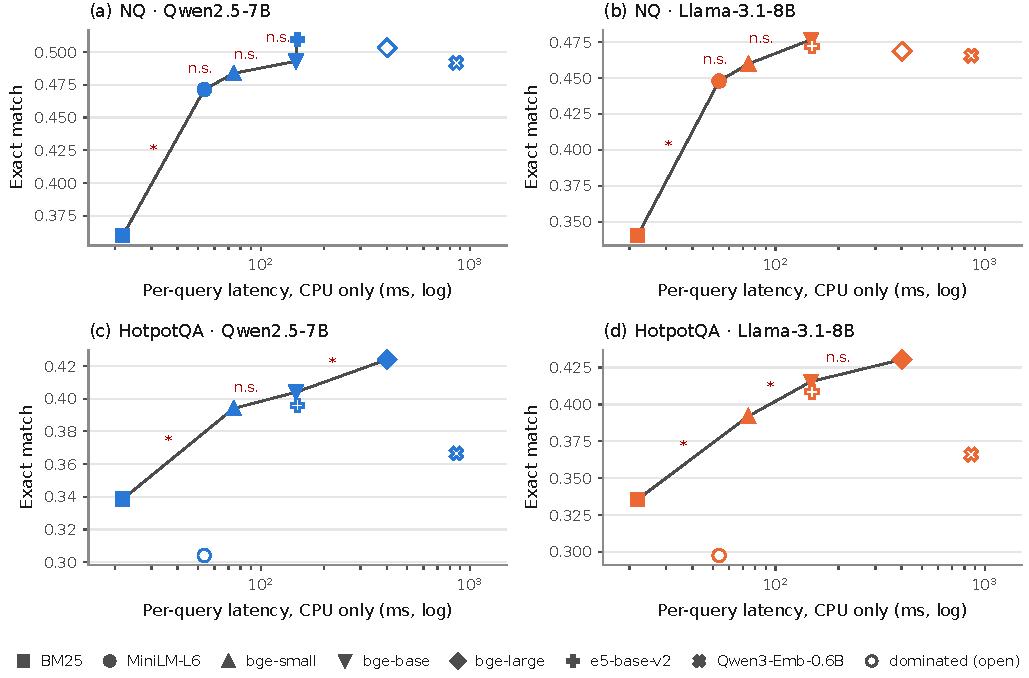
\includegraphics[width=\linewidth]{figs/fig11_pareto.pdf}
\caption{Exact match against per-query latency with query encoding and exact search on the CPU (Phase~1 cost measurements, log scale). The line joins retrievers that no other retriever beats on both axes; open markers are dominated. Step labels: $^{*}$ EM difference significant after Holm correction over the 21 pairs of the cell; n.s. not significant.}
\label{fig:pareto}
\end{figure}

\begin{table*}[t]
\centering
\footnotesize
\setlength{\tabcolsep}{3.5pt}
\caption{Deployment cost measured in Phase 1 (single measurements; one Tesla T4 and four virtual CPUs).}
\label{tab:deploy}
\begin{tabular}{lrrrrrrrr}
\toprule
Retriever & Enc.\ 300k (s) & GPU MiB & CPU pass./s & Q-enc GPU & Q-enc CPU & Search & Query CPU & Index MB \\
\midrule
BM25 & -- & -- & -- & -- & -- & 21.9 & 21.9 & -- \\
MiniLM-L6 & 158 & 352 & 38.7 & 5.6 & 14.3 & 39.3 & 53.7 & 439 \\
bge-small & 250 & 374 & 20.0 & 9.7 & 35.3 & 38.8 & 74.1 & 439 \\
bge-base & 584 & 818 & 6.4 & 9.6 & 66.5 & 81.2 & 147.7 & 879 \\
bge-large & 1,753 & 1,427 & 1.9 & 17.4 & 259.4 & 143.1 & 402.5 & 1,172 \\
e5-base-v2 & 592 & 818 & 6.2 & 9.6 & 67.8 & 81.5 & 149.3 & 879 \\
Qwen3-Emb-0.6B & 4,431 & 7,548 & 0.3 & 46.9 & 719.7 & 142.0 & 861.7 & 1,172 \\
\bottomrule
\end{tabular}
\par\smallskip\parbox{\linewidth}{\footnotesize Enc.\ 300k: T4 wall time to encode the 300,000-passage sub-corpus. Q-enc: batch-1 query encoding (ms, median). Search: batch-1 exact inner-product search on the CPU (ms, median). Query CPU: query encoding plus search, all on the CPU. Index: flat float32 FAISS index. Encoding throughput repeated five times in Phase 2 is in Table~\ref{tab:cost}.}
\end{table*}



\section{Additional tables}\label{app:tables}
Table~\ref{tab:ci} gives the bootstrap intervals for Table~\ref{tab:main}. Table~\ref{tab:transferalt} repeats the transfer ratios with token F1 and answer containment. Table~\ref{tab:decomp} gives EM given a hit and given a miss, which enter Eq.~\ref{eq:decomp}. Table~\ref{tab:idk} gives the abstention-prompt check, Table~\ref{tab:transferk} the exploratory transfer ratios at each $k$, Table~\ref{tab:pairwise} all pairwise EM tests, and Table~\ref{tab:judgerates} the excluded judge labels. Table~\ref{tab:components} gives the three decomposition terms with intervals, Table~\ref{tab:transdetail} the query-level transitions for two encoders, Table~\ref{tab:share} the HotpotQA shares under both orderings, and Table~\ref{tab:altbase} the ratios against BM25 and with Both@5.

\begin{table*}[t]
\centering
\small
\caption{95\% percentile bootstrap intervals (10,000 resamples over queries, seed 0) for the values in Table~\ref{tab:main}. Upper block: exact match per reader and dataset. Lower block: retrieval metrics, which do not depend on the reader.}
\label{tab:ci}
\begin{tabular}{lcccc}
\toprule
Condition & NQ Qwen & NQ Llama & HotpotQA Qwen & HotpotQA Llama \\
\midrule
BM25 & [0.340, 0.380] & [0.321, 0.360] & [0.318, 0.359] & [0.315, 0.356] \\
MiniLM-L6 & [0.451, 0.492] & [0.427, 0.469] & [0.284, 0.325] & [0.278, 0.318] \\
bge-small & [0.463, 0.505] & [0.439, 0.481] & [0.372, 0.415] & [0.370, 0.413] \\
bge-base & [0.473, 0.513] & [0.456, 0.497] & [0.383, 0.426] & [0.394, 0.438] \\
bge-large & [0.482, 0.524] & [0.448, 0.489] & [0.402, 0.446] & [0.408, 0.453] \\
e5-base-v2 & [0.489, 0.530] & [0.452, 0.493] & [0.374, 0.417] & [0.387, 0.430] \\
Qwen3-Emb-0.6B & [0.471, 0.512] & [0.445, 0.487] & [0.345, 0.388] & [0.345, 0.388] \\
Closed book & [0.135, 0.164] & [0.180, 0.213] & [0.143, 0.174] & [0.133, 0.165] \\
Gold passages & [0.633, 0.673] & [0.593, 0.633] & [0.607, 0.649] & [0.602, 0.645] \\
\midrule
Retrieval & NQ Hit@5 & & HotpotQA Hit@5 & HotpotQA Both@5 \\
\midrule
BM25 & [0.343, 0.383] & & [0.816, 0.849] & [0.244, 0.283] \\
MiniLM-L6 & [0.645, 0.683] & & [0.799, 0.834] & [0.212, 0.248] \\
bge-small & [0.710, 0.747] & & [0.944, 0.963] & [0.519, 0.563] \\
bge-base & [0.753, 0.788] & & [0.949, 0.967] & [0.550, 0.594] \\
bge-large & [0.779, 0.812] & & [0.952, 0.969] & [0.599, 0.642] \\
e5-base-v2 & [0.800, 0.832] & & [0.941, 0.960] & [0.522, 0.567] \\
Qwen3-Emb-0.6B & [0.726, 0.762] & & [0.934, 0.955] & [0.422, 0.467] \\
\bottomrule
\end{tabular}
\end{table*}

\begin{table*}[t]
\centering
\footnotesize
\caption{Components of the EM gain over MiniLM-L6 (Eq.~\ref{eq:decomp} multiplied by $\Delta\bar h$), with 95\% bootstrap intervals. Post hoc, descriptive.}
\label{tab:components}
\begin{tabular}{lcccc}
\toprule
Encoder & $\Delta$EM & Hit prevalence & EM among hits & EM among misses \\
\midrule
\multicolumn{5}{l}{\emph{NQ Qwen}} \\
bge-small & +0.012 & +0.022 [0.015, 0.029] & \ensuremath{-}0.012 [\ensuremath{-}0.026, 0.003] & +0.003 [\ensuremath{-}0.007, 0.012] \\
bge-base & +0.022 & +0.036 [0.028, 0.043] & \ensuremath{-}0.016 [\ensuremath{-}0.031, 0.000] & +0.002 [\ensuremath{-}0.007, 0.011] \\
bge-large & +0.032 & +0.044 [0.036, 0.052] & \ensuremath{-}0.013 [\ensuremath{-}0.029, 0.004] & +0.001 [\ensuremath{-}0.008, 0.009] \\
e5-base-v2 & +0.038 & +0.051 [0.043, 0.060] & \ensuremath{-}0.012 [\ensuremath{-}0.028, 0.005] & \ensuremath{-}0.001 [\ensuremath{-}0.009, 0.007] \\
Qwen3-Emb-0.6B & +0.020 & +0.027 [0.020, 0.034] & \ensuremath{-}0.009 [\ensuremath{-}0.024, 0.006] & +0.003 [\ensuremath{-}0.007, 0.012] \\
\multicolumn{5}{l}{\emph{NQ Llama}} \\
bge-small & +0.012 & +0.021 [0.014, 0.027] & \ensuremath{-}0.009 [\ensuremath{-}0.024, 0.006] & +0.000 [\ensuremath{-}0.009, 0.009] \\
bge-base & +0.029 & +0.034 [0.027, 0.041] & \ensuremath{-}0.012 [\ensuremath{-}0.028, 0.003] & +0.007 [\ensuremath{-}0.001, 0.016] \\
bge-large & +0.021 & +0.042 [0.034, 0.050] & \ensuremath{-}0.017 [\ensuremath{-}0.034, \ensuremath{-}0.002] & \ensuremath{-}0.004 [\ensuremath{-}0.012, 0.004] \\
e5-base-v2 & +0.024 & +0.048 [0.040, 0.057] & \ensuremath{-}0.024 [\ensuremath{-}0.040, \ensuremath{-}0.008] & \ensuremath{-}0.000 [\ensuremath{-}0.008, 0.008] \\
Qwen3-Emb-0.6B & +0.018 & +0.025 [0.019, 0.032] & \ensuremath{-}0.013 [\ensuremath{-}0.028, 0.003] & +0.005 [\ensuremath{-}0.004, 0.014] \\
\multicolumn{5}{l}{\emph{HotpotQA Qwen}} \\
bge-small & +0.090 & +0.034 [0.028, 0.041] & +0.058 [0.038, 0.078] & \ensuremath{-}0.003 [\ensuremath{-}0.005, \ensuremath{-}0.000] \\
bge-base & +0.100 & +0.035 [0.029, 0.042] & +0.066 [0.046, 0.087] & \ensuremath{-}0.002 [\ensuremath{-}0.004, 0.001] \\
bge-large & +0.120 & +0.036 [0.029, 0.043] & +0.085 [0.065, 0.105] & \ensuremath{-}0.001 [\ensuremath{-}0.003, 0.001] \\
e5-base-v2 & +0.092 & +0.034 [0.027, 0.040] & +0.062 [0.042, 0.082] & \ensuremath{-}0.003 [\ensuremath{-}0.005, \ensuremath{-}0.001] \\
Qwen3-Emb-0.6B & +0.062 & +0.032 [0.026, 0.039] & +0.031 [0.013, 0.050] & \ensuremath{-}0.001 [\ensuremath{-}0.003, 0.002] \\
\multicolumn{5}{l}{\emph{HotpotQA Llama}} \\
bge-small & +0.095 & +0.038 [0.031, 0.045] & +0.058 [0.038, 0.078] & \ensuremath{-}0.001 [\ensuremath{-}0.003, 0.001] \\
bge-base & +0.118 & +0.039 [0.033, 0.046] & +0.080 [0.059, 0.100] & \ensuremath{-}0.001 [\ensuremath{-}0.003, 0.001] \\
bge-large & +0.133 & +0.040 [0.033, 0.047] & +0.093 [0.073, 0.114] & \ensuremath{-}0.000 [\ensuremath{-}0.002, 0.002] \\
e5-base-v2 & +0.111 & +0.037 [0.031, 0.044] & +0.075 [0.056, 0.096] & \ensuremath{-}0.002 [\ensuremath{-}0.004, 0.001] \\
Qwen3-Emb-0.6B & +0.069 & +0.035 [0.029, 0.042] & +0.033 [0.015, 0.052] & +0.000 [\ensuremath{-}0.002, 0.003] \\
\bottomrule
\end{tabular}
\par\smallskip\parbox{\linewidth}{\footnotesize Hit prevalence: $\Delta\bar h\,(a_{R_1}-b_{R_1})$; EM among hits: $\bar h_R\,\Delta a$; EM among misses: $(1-\bar h_R)\,\Delta b$. The three terms add up to $\Delta$EM exactly. Intervals recompute every term in each resample.}
\end{table*}

\begin{table*}[t]
\centering
\footnotesize
\caption{Query-level transitions for bge-large and e5-base-v2 against MiniLM-L6. All 20 encoder--reader--dataset combinations are in the repository (transitions\_hit5.csv). Post hoc, descriptive.}
\label{tab:transdetail}
\begin{tabular}{lcccccc}
\toprule
Group & $n$ & EM MiniLM-L6 & EM encoder & wrong$\to$right / right$\to$wrong & Contribution & 95\% CI \\
\midrule
\multicolumn{7}{l}{\emph{NQ Qwen, bge-large}} \\
\quad miss $\to$ hit & 406 & 0.264 & 0.569 & 138 / 14 & +0.0550 & [0.0443, 0.0656] \\
\quad hit $\to$ hit & 1,389 & 0.588 & 0.567 & 71 / 99 & \ensuremath{-}0.0124 & [\ensuremath{-}0.0239, \ensuremath{-}0.0009] \\
\quad hit $\to$ miss & 108 & 0.537 & 0.333 & 5 / 27 & \ensuremath{-}0.0098 & [\ensuremath{-}0.0146, \ensuremath{-}0.0049] \\
\quad miss $\to$ miss & 352 & 0.233 & 0.227 & 21 / 23 & \ensuremath{-}0.0009 & [\ensuremath{-}0.0067, 0.0049] \\
\multicolumn{7}{l}{\emph{NQ Qwen, e5-base-v2}} \\
\quad miss $\to$ hit & 436 & 0.296 & 0.569 & 139 / 20 & +0.0528 & [0.0421, 0.0634] \\
\quad hit $\to$ hit & 1,405 & 0.588 & 0.569 & 66 / 92 & \ensuremath{-}0.0115 & [\ensuremath{-}0.0222, \ensuremath{-}0.0009] \\
\quad hit $\to$ miss & 92 & 0.522 & 0.370 & 3 / 17 & \ensuremath{-}0.0062 & [\ensuremath{-}0.0102, \ensuremath{-}0.0022] \\
\quad miss $\to$ miss & 322 & 0.186 & 0.208 & 20 / 13 & +0.0031 & [\ensuremath{-}0.0018, 0.0080] \\
\multicolumn{7}{l}{\emph{NQ Llama, bge-large}} \\
\quad miss $\to$ hit & 406 & 0.264 & 0.527 & 125 / 18 & +0.0475 & [0.0373, 0.0576] \\
\quad hit $\to$ hit & 1,389 & 0.552 & 0.534 & 64 / 89 & \ensuremath{-}0.0111 & [\ensuremath{-}0.0217, \ensuremath{-}0.0004] \\
\quad hit $\to$ miss & 108 & 0.583 & 0.287 & 4 / 36 & \ensuremath{-}0.0142 & [\ensuremath{-}0.0195, \ensuremath{-}0.0089] \\
\quad miss $\to$ miss & 352 & 0.207 & 0.199 & 20 / 23 & \ensuremath{-}0.0013 & [\ensuremath{-}0.0071, 0.0044] \\
\multicolumn{7}{l}{\emph{NQ Llama, e5-base-v2}} \\
\quad miss $\to$ hit & 436 & 0.268 & 0.525 & 133 / 21 & +0.0497 & [0.0390, 0.0603] \\
\quad hit $\to$ hit & 1,405 & 0.559 & 0.525 & 52 / 100 & \ensuremath{-}0.0213 & [\ensuremath{-}0.0319, \ensuremath{-}0.0111] \\
\quad hit $\to$ miss & 92 & 0.478 & 0.315 & 5 / 20 & \ensuremath{-}0.0067 & [\ensuremath{-}0.0111, \ensuremath{-}0.0022] \\
\quad miss $\to$ miss & 322 & 0.196 & 0.214 & 22 / 16 & +0.0027 & [\ensuremath{-}0.0027, 0.0080] \\
\multicolumn{7}{l}{\emph{HotpotQA Qwen, bge-large}} \\
\quad miss $\to$ hit & 307 & 0.098 & 0.414 & 106 / 9 & +0.0485 & [0.0385, 0.0590] \\
\quad hit $\to$ hit & 1,614 & 0.352 & 0.443 & 225 / 79 & +0.0730 & [0.0565, 0.0900] \\
\quad hit $\to$ miss & 20 & 0.150 & 0.000 & 0 / 3 & \ensuremath{-}0.0015 & [\ensuremath{-}0.0035, 0.0000] \\
\quad miss $\to$ miss & 59 & 0.102 & 0.102 & 1 / 1 & +0.0000 & [\ensuremath{-}0.0015, 0.0015] \\
\multicolumn{7}{l}{\emph{HotpotQA Qwen, e5-base-v2}} \\
\quad miss $\to$ hit & 290 & 0.107 & 0.383 & 85 / 5 & +0.0400 & [0.0310, 0.0495] \\
\quad hit $\to$ hit & 1,611 & 0.354 & 0.421 & 196 / 88 & +0.0540 & [0.0375, 0.0710] \\
\quad hit $\to$ miss & 23 & 0.087 & 0.000 & 0 / 2 & \ensuremath{-}0.0010 & [\ensuremath{-}0.0025, 0.0000] \\
\quad miss $\to$ miss & 76 & 0.066 & 0.040 & 0 / 2 & \ensuremath{-}0.0010 & [\ensuremath{-}0.0025, 0.0000] \\
\multicolumn{7}{l}{\emph{HotpotQA Llama, bge-large}} \\
\quad miss $\to$ hit & 307 & 0.072 & 0.397 & 107 / 7 & +0.0500 & [0.0400, 0.0605] \\
\quad hit $\to$ hit & 1,614 & 0.351 & 0.455 & 239 / 72 & +0.0835 & [0.0665, 0.1005] \\
\quad hit $\to$ miss & 20 & 0.100 & 0.050 & 1 / 2 & \ensuremath{-}0.0005 & [\ensuremath{-}0.0025, 0.0010] \\
\quad miss $\to$ miss & 59 & 0.068 & 0.068 & 0 / 0 & +0.0000 & [0.0000, 0.0000] \\
\multicolumn{7}{l}{\emph{HotpotQA Llama, e5-base-v2}} \\
\quad miss $\to$ hit & 290 & 0.079 & 0.417 & 105 / 7 & +0.0490 & [0.0390, 0.0590] \\
\quad hit $\to$ hit & 1,611 & 0.350 & 0.429 & 211 / 83 & +0.0640 & [0.0475, 0.0805] \\
\quad hit $\to$ miss & 23 & 0.217 & 0.043 & 1 / 5 & \ensuremath{-}0.0020 & [\ensuremath{-}0.0045, 0.0000] \\
\quad miss $\to$ miss & 76 & 0.040 & 0.040 & 0 / 0 & +0.0000 & [0.0000, 0.0000] \\
\bottomrule
\end{tabular}
\par\smallskip\parbox{\linewidth}{\footnotesize Intervals: percentile bootstrap over queries ($B=10{,}000$, seed 0); each query keeps its group, so group sizes vary across resamples and the interval is for the group's contribution to the population EM difference.}
\end{table*}

\begin{table}[t]
\centering
\small
\caption{Share of the HotpotQA EM gain over MiniLM-L6 that comes from changed conditional EM (percent), under the baseline-conditioned decomposition of Eq.~\ref{eq:decomp} with a 95\% bootstrap interval, and under the symmetric decomposition. Post hoc.}
\label{tab:share}
\begin{tabular}{lcccc}
\toprule
 & \multicolumn{2}{c}{Qwen reader} & \multicolumn{2}{c}{Llama reader} \\
\cmidrule(lr){2-3}\cmidrule(lr){4-5}
Encoder & Baseline-cond. & Symmetric & Baseline-cond. & Symmetric \\
\midrule
bge-small & 62 [49, 71] & 53 & 60 [47, 69] & 54 \\
bge-base & 64 [53, 73] & 57 & 67 [58, 74] & 60 \\
bge-large & 70 [62, 76] & 63 & 70 [63, 76] & 64 \\
e5-base-v2 & 64 [51, 72] & 54 & 67 [57, 74] & 60 \\
Qwen3-Emb-0.6B & 49 [26, 63] & 44 & 48 [28, 62] & 45 \\
\bottomrule
\end{tabular}
\par\smallskip\parbox{\linewidth}{\footnotesize Baseline-conditioned: $\Delta\mathrm{EM}=\Delta h\,(a_{R_1}-b_{R_1})+h_R\,\Delta a+(1-h_R)\,\Delta b$. Symmetric: each term averages the two orderings of the baseline and the encoder. Both identities hold exactly (residual $<10^{-12}$). The intervals resample queries ($B=10{,}000$, seed 0).}
\end{table}

\begin{table*}[t]
\centering
\small
\caption{Sensitivity of the transfer ratio to the baseline and to the retrieval metric, with 95\% bootstrap intervals. Upper block: $\Delta\mathrm{EM}/\Delta\mathrm{Hit@5}$ against BM25 instead of MiniLM-L6. Lower block: HotpotQA, $\Delta\mathrm{EM}/\Delta\mathrm{Both@5}$ against MiniLM-L6. Same queries, readers and reporting rule. Post hoc.}
\label{tab:altbase}
\begin{tabular}{lcccc}
\toprule
Encoder & NQ Qwen & NQ Llama & HotpotQA Qwen & HotpotQA Llama \\
\midrule
\multicolumn{5}{l}{\emph{Baseline BM25, denominator Hit@5}} \\
bge-small & 0.34 [0.29, 0.39] & 0.33 [0.28, 0.38] & 0.46 [0.31, 0.62] & 0.47 [0.31, 0.64] \\
bge-base & 0.33 [0.28, 0.37] & 0.34 [0.29, 0.38] & 0.52 [0.37, 0.69] & 0.64 [0.49, 0.81] \\
bge-large & 0.33 [0.29, 0.37] & 0.30 [0.25, 0.34] & 0.67 [0.51, 0.84] & 0.75 [0.59, 0.92] \\
e5-base-v2 & 0.33 [0.29, 0.37] & 0.29 [0.25, 0.33] & 0.49 [0.33, 0.66] & 0.62 [0.46, 0.80] \\
Qwen3-Emb-0.6B & 0.35 [0.30, 0.40] & 0.33 [0.28, 0.38] & 0.25 [0.09, 0.42] & 0.27 [0.12, 0.44] \\
\midrule
\multicolumn{5}{l}{\emph{Baseline MiniLM-L6, denominator Both@5}} \\
bge-small & -- & -- & 0.29 [0.23, 0.35] & 0.30 [0.24, 0.36] \\
bge-base & -- & -- & 0.29 [0.24, 0.35] & 0.34 [0.29, 0.40] \\
bge-large & -- & -- & 0.31 [0.26, 0.35] & 0.34 [0.29, 0.39] \\
e5-base-v2 & -- & -- & 0.29 [0.24, 0.35] & 0.35 [0.30, 0.41] \\
Qwen3-Emb-0.6B & -- & -- & 0.29 [0.21, 0.37] & 0.32 [0.24, 0.40] \\
\bottomrule
\end{tabular}
\par\smallskip\parbox{\linewidth}{\footnotesize BM25 with Both@5 is omitted: its Both@5 gain over MiniLM-L6 is 0.034 and its ratio is unstable (Qwen: 1.0 [0.5, 2.5]).}
\end{table*}

\begin{table*}[t]
\centering
\small
\caption{Transfer ratios with token F1 and answer containment in place of EM (same queries, baseline and reporting rule as Table~\ref{tab:transfer}).}
\label{tab:transferalt}
\begin{tabular}{lcccc}
\toprule
Retriever & NQ Qwen & NQ Llama & HotpotQA Qwen & HotpotQA Llama \\
\midrule
\multicolumn{5}{l}{\emph{Token F1}} \\
BM25 & 0.43 [0.37, 0.48] & 0.43 [0.37, 0.49] & n.e. & n.e. \\
bge-small & 0.26 [0.02, 0.49] & 0.23 [0.00, 0.45] & 0.76 [0.62, 0.92] & 0.85 [0.70, 1.01] \\
bge-base & 0.26 [0.11, 0.40] & 0.33 [0.19, 0.47] & 0.79 [0.65, 0.95] & 0.95 [0.80, 1.11] \\
bge-large & 0.27 [0.15, 0.39] & 0.25 [0.13, 0.36] & 0.97 [0.82, 1.14] & 1.10 [0.95, 1.28] \\
e5-base-v2 & 0.30 [0.20, 0.39] & 0.26 [0.17, 0.36] & 0.77 [0.62, 0.92] & 0.97 [0.82, 1.13] \\
Qwen3-Emb-0.6B & 0.26 [0.07, 0.45] & 0.29 [0.11, 0.47] & 0.52 [0.38, 0.66] & 0.66 [0.52, 0.81] \\
\multicolumn{5}{l}{\emph{Answer containment}} \\
BM25 & 0.45 [0.39, 0.52] & 0.46 [0.39, 0.52] & n.e. & n.e. \\
bge-small & 0.27 [0.01, 0.52] & 0.32 [0.07, 0.57] & 0.68 [0.53, 0.84] & 0.75 [0.61, 0.92] \\
bge-base & 0.34 [0.18, 0.49] & 0.38 [0.23, 0.53] & 0.72 [0.57, 0.88] & 0.90 [0.75, 1.07] \\
bge-large & 0.34 [0.21, 0.46] & 0.33 [0.21, 0.46] & 0.88 [0.73, 1.04] & 1.01 [0.86, 1.18] \\
e5-base-v2 & 0.36 [0.26, 0.47] & 0.33 [0.23, 0.43] & 0.71 [0.57, 0.87] & 0.91 [0.75, 1.07] \\
Qwen3-Emb-0.6B & 0.28 [0.08, 0.48] & 0.39 [0.20, 0.60] & 0.49 [0.35, 0.64] & 0.58 [0.45, 0.74] \\
\bottomrule
\end{tabular}
\end{table*}

\begin{table*}[t]
\centering
\small
\caption{Exact match given a hit and given a miss at Hit@5, $P(\mathrm{EM}\mid\mathrm{hit})$ / $P(\mathrm{EM}\mid\mathrm{miss})$, on the generation queries.}
\label{tab:decomp}
\begin{tabular}{lcccc}
\toprule
Retriever & NQ Qwen & NQ Llama & HotpotQA Qwen & HotpotQA Llama \\
\midrule
BM25 & 0.632 / 0.204 & 0.591 / 0.197 & 0.381 / 0.129 & 0.382 / 0.105 \\
MiniLM-L6 & 0.584 / 0.249 & 0.554 / 0.237 & 0.350 / 0.098 & 0.348 / 0.071 \\
bge-small & 0.568 / 0.259 & 0.542 / 0.239 & 0.411 / 0.043 & 0.409 / 0.043 \\
bge-base & 0.564 / 0.257 & 0.538 / 0.270 & 0.419 / 0.060 & 0.432 / 0.048 \\
bge-large & 0.568 / 0.252 & 0.533 / 0.220 & 0.438 / 0.076 & 0.446 / 0.063 \\
e5-base-v2 & 0.569 / 0.244 & 0.525 / 0.237 & 0.415 / 0.030 & 0.428 / 0.040 \\
Qwen3-Emb-0.6B & 0.572 / 0.260 & 0.538 / 0.256 & 0.383 / 0.090 & 0.383 / 0.072 \\
\bottomrule
\end{tabular}
\par\smallskip\parbox{\linewidth}{\footnotesize Closed-book EM for comparison: NQ 0.149 (Qwen), 0.197 (Llama); HotpotQA 0.158 (Qwen), 0.148 (Llama).}
\end{table*}

\begin{table}[t]
\centering
\small
\caption{Abstention prompt A3 (``I don't know'' allowed), Qwen reader, NQ, leading 200 queries of the seeded order (Phase 1).}
\label{tab:idk}
\begin{tabular}{lrcccccc}
\toprule
Context & $n$ & IDK rate & IDK $\mid$ hit ($n$) & IDK $\mid$ miss ($n$) & EM (A1) & EM (A3) & $p$ \\
\midrule
BM25 & 200 & 0.215 & 0.013 (79) & 0.347 (121) & 0.390 & 0.380 & 0.69 \\
MiniLM-L6 & 200 & 0.115 & 0.016 (124) & 0.276 (76) & 0.470 & 0.455 & 0.45 \\
bge-large & 200 & 0.045 & 0.024 (164) & 0.139 (36) & 0.495 & 0.465 & 0.07 \\
Gold passages & 200 & 0.060 & -- & -- & -- & -- & -- \\
\bottomrule
\end{tabular}
\par\smallskip\parbox{\linewidth}{\footnotesize $p$: exact McNemar test of EM under A3 against the main prompt A1, unadjusted.}
\end{table}

\begin{table*}[t]
\centering
\small
\caption{Exploratory: transfer ratio against MiniLM-L6 at each $k$, with Hit@$k$ matched to the $k$ passages the reader saw (Qwen reader, NQ, 2,255 queries; 95\% paired bootstrap intervals).}
\label{tab:transferk}
\begin{tabular}{lcccc}
\toprule
Retriever & $k=1$ & $k=3$ & $k=5$ & $k=10$ \\
\midrule
BM25 & 0.71 [0.61, 0.83] & 0.48 [0.41, 0.55] & 0.37 [0.31, 0.43] & 0.32 [0.26, 0.38] \\
bge-small & 0.83 [0.56, 1.22] & 0.37 [0.16, 0.59] & 0.19 [$-$0.07, 0.44] & 0.10 [$-$0.24, 0.42] \\
bge-base & 0.61 [0.45, 0.78] & 0.32 [0.19, 0.46] & 0.20 [0.04, 0.36] & 0.05 [$-$0.13, 0.22] \\
bge-large & 0.61 [0.47, 0.77] & 0.33 [0.22, 0.44] & 0.24 [0.11, 0.36] & 0.19 [0.02, 0.35] \\
e5-base-v2 & 0.57 [0.45, 0.69] & 0.32 [0.23, 0.41] & 0.25 [0.15, 0.36] & 0.05 [$-$0.09, 0.19] \\
Qwen3-Emb-0.6B & 0.41 [0.21, 0.60] & 0.35 [0.17, 0.53] & 0.25 [0.05, 0.45] & 0.08 [$-$0.27, 0.38] \\
\bottomrule
\end{tabular}
\par\smallskip\parbox{\linewidth}{\footnotesize Post hoc; the reporting rule of Section~\ref{sec:ratio} is not applied. For BM25 the ratio describes a retrieval loss.}
\end{table*}

\begin{table*}[t]
\centering
\small
\caption{Pairwise EM differences (row minus column) in every reader--dataset cell.}
\label{tab:pairwise}
\begin{tabular}{lrrrrrr}
\toprule
Row $-$ column & BM25 & MiniLM-L6 & bge-small & bge-base & bge-large & e5-base-v2 \\
\midrule
\multicolumn{7}{l}{\emph{NQ, Qwen}} \\
MiniLM-L6 & +0.112$^{*}$ &  &  &  &  &  \\
bge-small & +0.124$^{*}$ & +0.012 &  &  &  &  \\
bge-base & +0.133$^{*}$ & +0.022 & +0.009 &  &  &  \\
bge-large & +0.144$^{*}$ & +0.032$^{*}$ & +0.020 & +0.010 &  &  \\
e5-base-v2 & +0.150$^{*}$ & +0.038$^{*}$ & +0.026$^{*}$ & +0.016 & +0.006 &  \\
Qwen3-Emb-0.6B & +0.132$^{*}$ & +0.020 & +0.008 & $-$0.001 & $-$0.012 & $-$0.018 \\
\multicolumn{7}{l}{\emph{NQ, Llama}} \\
MiniLM-L6 & +0.108$^{*}$ &  &  &  &  &  \\
bge-small & +0.120$^{*}$ & +0.012 &  &  &  &  \\
bge-base & +0.137$^{*}$ & +0.029$^{*}$ & +0.017 &  &  &  \\
bge-large & +0.129$^{*}$ & +0.021 & +0.009 & $-$0.008 &  &  \\
e5-base-v2 & +0.132$^{*}$ & +0.024 & +0.012 & $-$0.004 & +0.004 &  \\
Qwen3-Emb-0.6B & +0.125$^{*}$ & +0.018 & +0.006 & $-$0.011 & $-$0.003 & $-$0.007 \\
\multicolumn{7}{l}{\emph{HotpotQA, Qwen}} \\
MiniLM-L6 & $-$0.035$^{*}$ &  &  &  &  &  \\
bge-small & +0.056$^{*}$ & +0.090$^{*}$ &  &  &  &  \\
bge-base & +0.066$^{*}$ & +0.100$^{*}$ & +0.010 &  &  &  \\
bge-large & +0.086$^{*}$ & +0.120$^{*}$ & +0.030$^{*}$ & +0.020$^{*}$ &  &  \\
e5-base-v2 & +0.058$^{*}$ & +0.092$^{*}$ & +0.002 & $-$0.008 & $-$0.028$^{*}$ &  \\
Qwen3-Emb-0.6B & +0.028$^{*}$ & +0.062$^{*}$ & $-$0.028$^{*}$ & $-$0.037$^{*}$ & $-$0.058$^{*}$ & $-$0.029$^{*}$ \\
\multicolumn{7}{l}{\emph{HotpotQA, Llama}} \\
MiniLM-L6 & $-$0.038$^{*}$ &  &  &  &  &  \\
bge-small & +0.057$^{*}$ & +0.095$^{*}$ &  &  &  &  \\
bge-base & +0.080$^{*}$ & +0.118$^{*}$ & +0.024$^{*}$ &  &  &  \\
bge-large & +0.095$^{*}$ & +0.133$^{*}$ & +0.038$^{*}$ & +0.015 &  &  \\
e5-base-v2 & +0.073$^{*}$ & +0.111$^{*}$ & +0.017 & $-$0.007 & $-$0.022$^{*}$ &  \\
Qwen3-Emb-0.6B & +0.030$^{*}$ & +0.069$^{*}$ & $-$0.026$^{*}$ & $-$0.050$^{*}$ & $-$0.065$^{*}$ & $-$0.043$^{*}$ \\
\bottomrule
\end{tabular}
\par\smallskip\parbox{\linewidth}{\footnotesize $^{*}$: exact McNemar test significant after Holm correction over the 21 pairs of the cell ($p<0.05$).}
\end{table*}

\begin{table}[t]
\centering
\small
\caption{Phase~1 LLM-judge labels (Mistral-7B-Instruct-v0.3, zero-shot prompt of Appendix~\ref{app:judge}), Qwen reader, NQ. \textbf{Excluded from all conclusions} because agreement with human labels was slight ($\kappa$ = 0.127).}
\label{tab:judgerates}
\begin{tabular}{lrc}
\toprule
Context & $n$ & Share judged SUPPORTED [95\% CI] \\
\midrule
BM25 & 500 & 0.790 [0.754, 0.826] \\
MiniLM-L6 & 500 & 0.886 [0.858, 0.914] \\
bge-small & 500 & 0.898 [0.870, 0.924] \\
bge-base & 500 & 0.902 [0.876, 0.928] \\
bge-large & 500 & 0.912 [0.886, 0.936] \\
e5-base-v2 & 500 & 0.916 [0.890, 0.940] \\
Qwen3-Emb-0.6B & 500 & 0.896 [0.870, 0.922] \\
Gold passages & 499 & 0.966 [0.950, 0.980] \\
\bottomrule
\end{tabular}
\par\smallskip\parbox{\linewidth}{\footnotesize 3,999 judgements; one gold-passage output reached the token limit, so the gold row has 499 items.}
\end{table}


\begin{figure}[t]
\centering
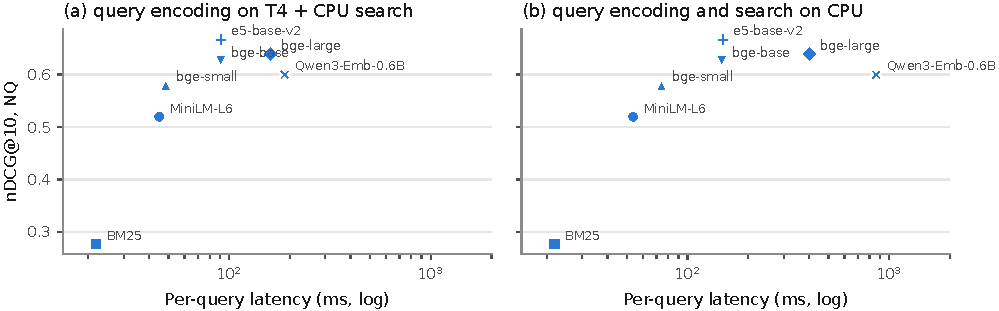
\includegraphics[width=\linewidth]{figs/fig12_latency.pdf}
\caption{NQ nDCG@10 against per-query latency (Phase~1 batch-1 medians, log scale): (a) query encoding on the T4 and exact search on the CPU; (b) both on the CPU.}
\label{fig:latency}
\end{figure}
